\documentclass[12pt, a4paper, oneside, ngerman]{article}
\usepackage[utf8]{inputenc}
\usepackage[T1]{fontenc}
\usepackage[]{hyperref}
\usepackage{graphicx}
\usepackage{listings}
\usepackage{caption}
\usepackage{algorithm2e}


\title{Projektarbeit Compilerbau}
\usepackage[german]{babel}

\setlength\parindent{0pt}

\begin{document}
\selectlanguage{german}
\author{Jonas Wenner, Jens Marvin Reuter, Noah Hoffmann}

\maketitle
\thispagestyle{empty}
\pagebreak
\tableofcontents
\newpage


\begin{abstract}

\noindent
Als Abschlussprojekt des Moduls 'Compilerbau' unter Leitung von Thorsten Jakobs, M.Sc., htw saar wurde dieser Compiler zur von uns eigens entwickelten Sprache \textit{UCBS} (\textbf{U}nsere \textbf{C}ompiler\textbf{b}au-\textbf{S}prache) entwickelt, mit den in \textit{\ref{sec:anforderungen}. Anforderungen} beschriebenen Voraussetzungen und Zielen. Die Sprache besitzt eine C-ähnliche Syntax, wurde jedoch auf wesentliche Elemente wie Grundrechenarten, Funktionen, if-Statements und eine Form der Schleife reduziert. Weiterhin vorhanden sind Bezeichner, Konstanten und Variablen. Die Klammerung wird ebenfalls berücksichtigt.
\\\\
Diese Dokumentation behandelt die Anforderungen an den Compiler, den theoretischen Hintergrund, die Konzeption der Entwicklung, unsere verwendeten Technologien, sowie unsere Vorgehensweise während der Entwicklung und die Probleme, auf die wir gestoßen sind und unsere Lösungsansätze. Ausgangs wird auch die Handhabung des Compilers näher erläutert.

\end{abstract}

\newpage
% !TEX root = Main.tex

\section{Anforderungen}
\label{sec:anforderungen}
Um zu gewährleisten, dass alle Modulteilnehmer über die gleichen Voraussetzungen verfügen und nach festgelegten Kriterien bewertet werden können, wurden durch den Modulverantwortlichen einige Rahmenbedingungen vorgegeben. Die Prüfleistung besteht dabei aus der Entwicklung einer einfachen Programmiersprache, dem Anfertigen einer Dokumentation sowie der Präsentation der Ergebnisse. Die Anforderungen an das Projekt werden in den folgenden Abschnitten aufgeführt und erläutert.

\subsection{Infrastruktur}
Das Ziel ist die Enwicklung eines Compiler-Frontends, welches Quelltext in der von uns entwickelten Programmiersprache zu Jasmin-Code übersetzt. 
Jasmin ist ein Assembler für die Java Virtual Machine, der Quelltext in einer Assembler-ähnlichen Syntax zu Bytecode übersetzt. 
Dieser Bytecode kann schließlich von der Java Virtual Machine ausgeführt werden.


\subsection{Programmiersprache}
Die von uns entwickelte Programmiersprache besitzt folgende Komponenten: 
\begin{itemize}
\item Bezeichner
\item Konstanten
\item Variablen
\item Arithmetik mit Grundrechenarten
\item Klammerung
\item Funktionen
\item if-else-Anweisung
\item while-Schleife
\end{itemize}

Die Entwicklung wird mit 50\% in der Gesamtbewertung gewichtet.
In einem späteren Kapitel dieser Dokumentation wird erläutert, wie die Programmiersprache verwendet wird.

\subsection{Dokumentation}
Es ist eine Dokumentation anzufertigen, die Aufschluss über die Konzeption der Entwicklung, die verwendeten Technologien, das Vorgehen während der Entwicklung, aufgetretene Probleme und Lösungsansätze zu diesen sowie die Verwendung des Compilers gibt.

Die Dokumentation wird mit 30\% in der Gesamtbewertung gewichtet.

\subsection{Präsentation}
In einer circa 20-minütigen Präsentation werden die verwendeten Technologien, wichtige Entwicklungsschritte, sowie aufgetretene Probleme erläutert. Außerdem wird der Compiler vorgeführt. 

Die Präsentation wird mit 20\% in der Gesamtbewertung gewichtet.

\pagebreak
% !TEX root = Main.tex

\section{Theoretischer Hintergrund}
Um die folgenden Abschnitte verständlich zu machen ist eine kurze Erläuterung des theoretischen Hintergrunds sinnvoll.
\subsection{Verallgemeinerung}
Der zu entwickelnde Compiler nimmt als Eingabe eine Text-Datei mit Instruktionen in der Ausgangssprache. Der Compiler verarbeitet diese Eingabe und gibt als Ausgabe eine Datei mit Anweisungen in der Zielsprache zurück. Diese Verarbeitung kann grob in drei Abschnitte eingeteilt werden.
\subsection{Lexikalische Analyse}
Der erste Schritt ist dabei die sogenannte lexikalische Analyse. Die Eingabedatei ist für den Computer zunächst nur eine Kette von Zeichen. Diese Zeichen sind in sogenannte Tokens aufzuteilen. Beispielhaft könnte die Eingabe
\begin{lstlisting} [frame=single]
 a = b + c;
\end{lstlisting}

zu den folgenden Tokens aufgelöst werden.


\begin{figure}[h!]
\centering
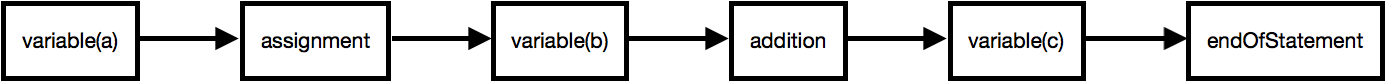
\includegraphics[scale=0.5]{pics/lex_beispiel.png}
\caption{Kurzes Beispiel für lexikalische Analyse}

\end{figure}

Der Teil des Compilers, der diese Aufgabe übernimmt, wird \textit{Lexer} genannt. Der Lexer überprüft für jedes Zeichen der Eingabedatei, welchem Token dieses zugeordnet werden kann. Dies geschieht auf Grundlage von definierten Regeln, welche mit sogenannten \textit{regulären Ausdrücken} formuliert werden. Ein regulärer Ausdruck besteht aus einer Sequenz von Zeichen, die ein bestimmtes Muster definieren. Reguläre Ausdrücke können auch rekursiv verwendet werden, um auf Grundlage einfacher regulärer Ausdrücke komplexere zu bilden. Beispiele für reguläre Ausdrücke werden im Kapitel \textit{\ref{subsec:arithExp}. Erste Schritte: Auswertung von arithmetischen Ausdrücken} aufgeführt.

\subsection{Syntaktische Analyse}
% TO-DO: Grafik
Im zweiten Schritt der Verarbeitung wird die \textit{syntaktische Analyse} durchgeführt. Dabei wird überprüft, ob die Eingabedatei einer definierten Grammatik entspricht, während bei der lexikalischen Analyse lediglich die übergebene Zeichenfolge in Tokens aufgeteilt wird, nicht jedoch überprüft wird, ob diese der Grammatik entsprechend zusammengeführt werden können. 

Bei einer erfolgreichen Auswertung wird die Folge an Tokens, die bei der lexikalischen Analyse ermittelt wurde, in einen Syntaxbaum übergeführt. Dies ist notwendig, um die Tokens in der richtigen Reihenfolge auszuwerten. 
%hier wäre eine Grafik auch hilfreich
%ich kümmere mich drum  -- lg marvin

\subsection{Syntaxgesteuerte Übersetzung}
Die eigentlich Erzeugung von Code in der Ausgangssprache findet zuletzt statt. Hierbei wird jeder Knoten des Syntaxbaum betrachtet und je nach Kontext eine Zeichenkette mit Anweisungen in der Zielsprache generiert. In diesem Schritt findet ebenfalls die semantische Analyse statt, beispielsweise die Überprüfung, ob eine aufgerufene Variable vorher deklariert wurde.

\pagebreak
\section{Konzeption der Entwicklung}
\subsection{Allgemeiner Grundsatz}
\label{sec:grundsatz}
Während der Entwicklung versuchten wir uns möglichst kleine Zwischenziele zu setzen, um die Aufgabe in überschaubare, einfach zu lösende Teilprobleme zu unterteilen. Rückblickend war dies eine sinnvolle Strategie, die zum gewünschten Ziel führte.
% !TEX root = Main.tex

\subsection{Wahl der Entwicklungswerkzeuge}
Bezüglich der Entwicklungswerkzeuge wurden uns verschiedene Möglichkeiten vorgestellt. Die erste Möglichkeit bestand darin das Tool ''lex'' beziehungsweise dessen Open-Source-Implementierung ''flex'' als Lexer-Generator und das Tool ''yacc'' beziehungsweise dessen Open-Source-Implementierung ''bison'' als Parser-Generator zu nutzen. Die zweite Möglichkeit bestand in der Nutzung des Werkzeuges ANTLR, das die Funktionalitäten der zuvor genannten Werkzeuge in einem Programm zusammenfasst.

Da ANTLR automatisiert auf Grundlage einer Datei, die die von uns formulierte Grammatik der Sprache enthält, Lexer sowie Parser zeitgleich erstellen kann, entschieden wir uns für diese Variante. Der Vorteil besteht dabei darin, dass zwei essentielle Teile des Compilers von einem Tool übernommen werden. 

\subsection{Herkunft des Namens C=}
Für die Programmiersprache wurde der Name C= gewählt (gesprochen: C equal). Ursprünglich sollte die Programmiersprache C - - genannt werden, in Anlehnung an den verkleinerten Sprachumfang der Sprache C sowie der Namensgebung von C++. Da C - - jedoch bereits als Zwischensprache existiert, wurde die im Rahmen des Moduls Compilerbau entwickelte Sprache in Anlehnung an C\# (\# ist auch als vier aneinandergereihte Additionssymbole zu interpretieren) C= genannt, wobei das = vier aneinandergereihte Subtraktionszeichen darstellt.

\subsection{Sprachdesign}
Es wurde sich darauf geeinigt, dass die Syntax der von uns entworfenen Ausgangssprache der Syntax der Programmiersprache C ähnlich sein soll, da dies gleich mehrere Vorteile hervorbringt:
\begin{itemize}
\item Alle Projektteilnehmer sind mit der Sprache C vertraut
% Was bedeutet "compilierte Sprache" in diesem Zusammenhang? Bitte um Aufklärung - der nohoffmann
\item C ist eine der am weitesten verbreiteten compilierten Sprachen
%\item Die Sprache C besitzt aufgrund seiner Klammerregeln, sowie anderer sprachlicher Regeln und Konventionen eine gute Lesbarkeit
% Die Konventionen haben ja eher wenig mit dem Sprachdesign zu tun (oder?)
% vllt eher:
\item Quellprogramme in C-Syntax besitzen eine gute Lesbarkeit
\end{itemize}

\subsection{Implementierung}
Unser Compiler verwendet im Zusammenspiel mit dem von ANTLR generierten Lexer und Parser einen Visitor für die syntaxgesteuerte Übersetzung. Die Alternative dazu besteht in einem Listener, der sich von einem Visitor dahingehend unterscheidet, dass die verschiedenen Methoden die auf die Knoten des Syntaxbaumes angewandt werden, keinen Rückgabewert besitzen und die Ergebnisse dieser somit seperat gespeichert werden müssen. Der Vorteil eines Listeners hingegen besteht darin, dass untergeordnete Knoten im Syntaxbaum automatisch bearbeitet werden und nicht wie beim Visitor explizit besucht werden müssen. Nach der Abwägung dieser Vor- und Nachteile entschieden wir uns für einen Visitor, da dieser uns als die effizientere Methode erschien.




\pagebreak
% !TEX root = Main.tex

\section{Verwendete Technologien}

\subsection{Eclipse}
Zur Entwicklung wurde die integrierte Entwicklungsumgebung Eclipse in der aktuellen Version (4.8.0) genutzt. 
Eclipse bietet mehrere Vorteile, die ein einfacheres und effizienteres Entwickeln erlauben. Eclipse enthält einen Datei-Explorer, mit dessen Hilfe die Navigation durch die verschiedenen Verzeichnisse zusammen mit Editor und Konsole innerhalb eines Fensters geschehen kann. Des Weiteren bietet Eclipse automatische Vorschläge zur Code- und Textvervollständigung an, was die Schreibgeschwindigkeit und damit die Arbeitseffizienz erhöht. 
Außerdem kann Eclipse durch Plug-Ins erweitert werden. Als Plug-In nutzen wir beispielsweise das Test-Framework TestNG, um verschiedene Testfälle automatisiert zu prüfen.
\\\\
Ein großer Nachteil von Eclipse ist die Unzuverlässigkeit. Die IDE wirft immer wieder nicht nachvollziehbare, manchmal sogar gar keine Fehlermeldungen. Des weiteren trat unabhängig voneinander auf verschiedenen Rechnern mit verschiedenen Betriebssystemen (getestet u.A. unter Ubuntu Linux, Arch Linux und Mac OS X) das Problem auf, dass das Projekt nicht geöffnet werden konnte. Besonders kafkaesk war jedoch die Situation, dass sich das Projekt mit der \textit{'Eclipse IDE for C/C++ Developers'} öffnen ließ. Letzendlich war die Arbeit mit Eclipse unter Arch Linux nicht möglich, sodass andere Projektteilnehmer die Aufgabe des Kompilierens übernehmen mussten.

\subsection{TestNG}
% TO-DO: Versionsnummer prüfen
TestNG ist ein Framework, das dem zu testenden Programm Eingabewerte übergibt und die tatsächlichen Ergebnisse des Programms mit den erwarteten Ergebnissen abgleicht. Dabei können beliebig viele Testszenarien geprüft werden. Es werden sogenannte positive Tests, also solche, bei denen die Eingabe ein erwartetes Ergebnis hervorruft, als auch negative Tests, bei denen geprüft wird, ob nicht vorhergesehene Eingaben mit entsprechenden Fehlermeldungen korrekt behandelt werden, durchgeführt. TestNG wurde von uns in Version 6.10 (PRÜFEN!) genutzt.

Als Beispiel: Der Quelltext
\begin{lstlisting} [frame=single]
println(1+4);
\end{lstlisting}

sollte als Ergebnis ''5'' auf der Konsole ausgeben. TestNG übergibt den Quelltext an unseren Compiler, ruft Jasmin auf, führt das Programm aus und gleicht dann die Ergebnisse ab. Wenn das Ergebnis ''5'' ist, gilt der Test als bestanden, andernfalls als durchgefallen. 

\subsection{ANTLR}
ANTLR steht für \textit{ANother Tool for Language Recognition} und ist ein Lexer- und Parsergenerator. ANTLR generiert auf Grundlage einer Grammatik-Datei Java-Code, der einen entsprechenden Lexer sowie ein Template für Teile des Parsers implementiert. Dadurch, dass die von ANTLR generierten Programme aus einer Eingabedatei in der Ausgangssprache einen Syntaxbaum erstellen können, besteht der größte Arbeitsaufwand daraus, Grammatiken für ANTLR zu formulieren und Teile des Parsers (in unserem Fall ein Visitor) zu implementieren. Es wurde die ANTLR-Version 4.7.1 verwendet.

\subsection{Jasmin}
Jasmin ist ein Assembler für die Java Virtual Machine. Dabei werden Textdateien mit Anweisungen in Jasmin-Syntax zu Bytecode übersetzt. Dieser Bytecode kann von der JVM ausgeführt werden.

\subsection{Java}
% TO-DO: Finalen Namen der Sprache einfügen
Die Programmiersprache Java wurde für das Projekt gewählt, da der von ANTLR generierte Code ebenfalls in Java ist. Es ist teilweise notwendig von Klassen des ANTLR generierten Code abzuleiten, weshalb die Wahl einer anderen Programmiersprache als Java Problemstellungen wie die Code-Kompatibilität zur anderen Programmiersprache darstellt. 
Des Weiteren muss die Java Runtime Environment ohnehin genutzt werden, um ANTLR, Jasmin sowie schließlich die Kompilate des C=-Compilers auszuführen.

\subsection{Java Virtual Machine}
Die Java VM ist ein Zwischenschritt beim Ausführen von Java-Code. Eine Java-Quelldatei (.java) wird zunächst durch den Java-Compiler zu Bytecode (.class) übersetzt und dann von der Java VM interpretiert. Dieser Zwischenschritt ermöglicht eine Plattformunabhängigkeit, da die Kompilate (.class-Dateien) nicht maschinenspezifisch übersetzt werden. Plattformabhängiger Maschinencode wird erst von der Java VM generiert, weshalb jeder Bytecode ausgeführt werden kann, solange für die entsprechende Maschine die Java VM verfügbar ist.
% ToDo : Java generiert keinen Maschinenspezifischen Bytecode: JavaVM liest den Maschinenunabhängigen Bytecode Byte für Byte aus und kann dann evtl. Maschinenabhängig interpretieren. Ist Quasi ab hier wie eine Interpretersprache. Interpreter bekommt maschinenunabhängigen Code und weiss dann, wie er auf der Maschine auszuführen ist, dass das Ergebnis gleich bleibt.

In diesem Projekt wird die Java VM jedoch nicht nur zur Übersetzung unseres Code genutzt, sondern auch um die Kompilate unseres eigenen Compilers auszuführen. Diese Kompilate werden von Jasmin zu Bytecode übersetzt, der Bytecode wiederum wird von der Java VM ausgeführt.

% ToDo : Doppelt????

Zu beachten ist, dass die Java VM stack-basiert operiert und nicht wie beispielsweise der x86-Befehlssatz mit Registern arbeitet, was bei der Implementierung zu beachten ist und eine besondere Denkweise erfordert. 

\subsection{Git}
Nach einiger Zeit der Arbeit am Projekt wurde klar, dass es auf Dauer sehr ineffizient ist, die Aktualisierungen über eine WhatsApp-Gruppe zu verteilen. Daher haben wir über die Plattform \textit{GitHub} ein Repository erstellt. Die Arbeit über das Webinterface auf github.com sowie mit der 'GitHub Desktop'-App lief störungsfrei.
\pagebreak
% !TEX root = Main.tex

\section{Vorgehen während der Entwicklung}
\subsection{Erste Schritte: Auswertung von arithmetischen Ausdrücken}
\label{subsec:arithExp}
% TO-DO: Kapitelnummer einfügen und prüfen
% kapitel 5 ist hier doch falsch????
Der Vorgehensweise unter \textit{\ref{sec:grundsatz}. Allgemeiner Grundsatz} entsprechend, implementierten wir zuerst die unserer Sicht nach grundlegendste Fähigkeit einer Programmiersprache: das Auswerten von arithmetischen Ausdrücken. Es soll möglich sein, Ausdrücke, die die Grundrechenarten sowie eine beliebig tiefe Schachtelung von Klammern enthalten, zu erkennen und der Operatorenpriorität entsprechend die gelesenen Tokens in einem Syntaxbaum zusammenzuführen. Dazu formulierten wir folgende Grammatik:


\scriptsize\begin{lstlisting} [frame=single] 
//Datei: Arithmetic.g4
grammar Arithmetic;

///////////////////////////////////////////////////////
// beliebige Folge der Ziffern 0 bis 9
INTEGER : [0-9]+ ;        
// ueberspringt Leerzeichen, Tabstops sowie Linefeeds
WS : [ \t\r\n]+ -> skip ; 
// oeffndende runde Klammer
LPAREN : '(';		  	  
// schliessende runde Klammer
RPAREN : ')';		  	  
///////////////////////////////////////////////////////
//mathematische Operatoren
PLUSOP : '+';
MINOP : '-';
MULTOP : '*';
DIVOP : '/';
///////////////////////////////////////////////////////
//Regeln fuer math. Ausdruecke
expression: INTEGER					
	| LPAREN expression RPAREN		
	| expression DIVOP  expression  
	| expression MULTOP expression	
	| expression MINOP  expression 
	| expression PLUSOP expression 
	;			
///////////////////////////////////////////////////////

\end{lstlisting}
\normalsize
Eine Grammatik für ANTLR hat folgenden Aufbau:

Die Definition der Grammatik beginnt mit dem Schlüsselwort ''grammar'' sowie dem Namen der Grammatik. Dabei gilt es zu beachten, dass die Datei den gleichen Namen wie die Grammatik selbst sowie die Dateiendung ''.g4'' besitzt. Diese Deklaration wird mit einem Semikolon abgeschlossen.

Zeilen, die mit ''//'' beginnen, sind Kommentare und haben keinen Einfluss auf die Grammatik. Sie dienen lediglich als Erläuterungen und zur Formatierung, um die Lesbarkeit zu verbessern.

Auf die Deklaration dürfen beliebig viele Regeln für die Grammatik folgen. Zur Formulierung der Regeln werden reguläre Ausdrücke genutzt. Beispielsweise besagt die sechste Zeile, dass es eine Regel INTEGER gibt, wobei ein INTEGER sich aus einer beliebigen Folge der Ziffern von 0 bis 9 zusammensetzt. Der reguläre Ausdruck [0-9] gibt an, dass ein beliebiges Zeichen im Bereich von 0 bis 9 vorkommen darf. Das abschließende ''+'' bedeutet, dass es sich um eine Kette dieser Zeichen, die beliebig lange ist, jedoch mindestens die Länge 1 besitzt, handelt.

Die Regel WS (Whitespace) besagt, dass bestimmte Zeichen, die nur der Formatierung dienen, ignoriert werden, da sie für das Übersetzen einer Quelldatei keine Bedeutung haben.

Die darauffolgenden Regeln sind Aliase für die Zeichen, die in arithmetischen Ausdrücken verwendet werden. Diese Auslagerung steigert unseres Erachtens nach die Lesbarkeit der letzten Regeln dieses Beispiels, sind aber nicht zwingend notwendig.

Die wohl relevanteste Regel trägt den Namen ''expression'' und legt fest, wie sich ein arithmetischer Ausdruck zusammensetzen kann. Im Vergleich zu den vorherigen Regeln, wurde hier von der Möglichkeit, mehrere alternative Möglichkeiten anzugeben, Gebrauch gemacht. Die Regel besagt, dass ein arithmetischer Ausdruck entweder aus 
\begin{itemize}
\item einer Zahl,
\item einem geklammerten Ausdruck,
\item einer Division mit zwei Operanden,
\item einer Multiplikation mit zwei Operanden,
\item einer Subtraktion mit zwei Operanden
\item oder einer Addition mit zwei Operanden
\end{itemize}
besteht.
Durch die Rekursion (die Regel verweist auf sich selbst) ist eine beliebige Länge des Ausdruckes möglich.

Eine Besonderheit, die zu beachten ist, besteht in der Rangfolge der Operatoren. Die höchste Bindung besitzt ein geklammerter Term, die nächst höchste Bindung Divisionen und Multiplikationen. Die schwächste Bindung besitzen Subtraktionen und Additionen.

Damit diese Priorität gewährleistet werden kann, sind die Regeln in dieser bestimmten Reihenfolge notiert. ANTLR versucht immer zuerst die ''oberste'' Regel anzuwenden, daraufhin die darunter stehende usw.. Deshalb wird der folgende Ausdruck 

\begin{lstlisting} [frame=single]
2*10-48*(4-1)-16/4
\end{lstlisting}

zu diesem Syntaxbaum aufgelöst:

\begin{figure}[h!]
\centering
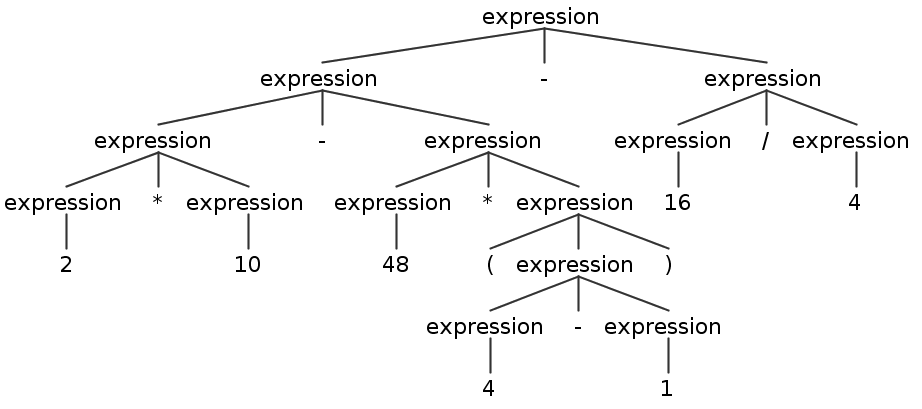
\includegraphics[scale=0.4]{pics/antlr4_parse_tree_arithmetic.png}
\caption{Syntaxbaum für beispielhaften arithmetischen Ausdruck}
\end{figure}

Des Weiteren ist zu beachten, dass arithmetischen Ausdrücke gleicher Operatorenpriorität von links  nach rechts ausgewertet werden müssen. Als Beispiel lässt sich hier der Term 
\begin{lstlisting} [frame=single]
8-5+2
\end{lstlisting}
nennen. Sowohl die Subtraktion als auch die Addition besitzen die gleiche Bindung. Wenn man hier fälschlicherweise zuerst die Addition, also 5+2, was 7 ergibt, auswertet und das Ergebnis dieser Operation von 8 subtrahiert, erhält man als Gesamtergebnis 1. 
In der korrekten Reihenfolge erfolgt zuerst die Subtraktion, also 8-5, was 3 ergibt, und erst darauf die Addition von 1, was als Gesamtergebnis 4 liefert. 
Um diese Fehlerquelle auszuschließen, sind in unserer Grammatik die Regel für Subtraktion vor der für Addition und die Regel für Division vor der für Multiplikation definiert. Da bei reinen Additionen bzw. reinen Multiplikationen die Auswertungsreihenfolge tatsächlich keine Rolle spielt, eine Subtraktion jedoch vor einer Additionen (vgl. Beispiel oben) ausgewertet werden muss, sorgt die Reihenfolge der Regeln in der Grammatik für eine korrekte Auswertung.

Ein analoges Beispiel zu Divisionen und Multiplikationen ist
\begin{lstlisting} [frame=single]
8/2*4
\end{lstlisting}
Auch hier ergibt sich ein ähnliches Problem wie beim vorherigen Beispiel. Wird zuerst die Multiplikation (2*4) ausgeführt und erst danach die Division (also 8/8 in diesem Fall), ist das Endergebnis 1 und nicht wie in der richtigen Reihenfolge 16.

Nach diesen Schritten sind wir also in der Lage einen Syntaxbaum zu erstellen. Der nötige Programmcode dafür wird von ANTLR automatisiert erstellt. Dabei ist die Eingabe dieses Programmes der auszuwertende Ausdruck. Die Ausgabe ist der Syntaxbaum, der zu Testzwecken auch als Grafik (vgl. Abbildung oben) ausgegeben werden kann. 

Der nächste wichtige Schritt der Übersetzung besteht nun in der Auswertung dieses Baumes. Dazu wird der Baum als Datenstruktur betrachtet. ANTLR liefert dabei mehrere Methoden, die auf Instanzen der Klasse ''ParseTree'' angewandt werden können. 
Jedes Token, das in der Grammatik definiert wurde und durch einen Knoten im Baum repräsentiert wird, besitzt eine sogenannte Visit-Methode. Diese Methode gibt eine Kette mit Zeichen zurück, wobei diese Zeichenkette die Anweisungen in der Zielsprache (Jasmin) enthält. Das Abarbeiten dieser Visit-Methoden in der richtigen Reihenfolge bildet die Grundlage für die Übersetzung, da hiernach alle Instruktionen in der Zielsprache zusammengesetzt sind. Was genau in einer Visit-Methode passiert, wird vom Entwickler festgelegt. ANTLR stellt sogehesen nur eine Vorlage zur Verfügung.

Um diese korrekte Reihenfolge zu gewährleisten, muss eine Anfangsregel (Startaxiom) festgelegt sein. In diesem Beispiel wurde festgelegt, dass der Programmstart - sprich der Wurzelknoten des Baumes - eine ''expression'' sein muss. Das bedeutet, das zunächst die Visit-Methode des Wurzelknoten aufgerufen wird. Damit nun auch die inneren Knoten des Syntaxbaums berücksichtigt werden, ist der Aufruf einer weiteren von ANTLR generierten Methode notwendig. Jeder Knoten des Baum besitzt eine visitChildren()-Methode, welche die entsprechenden Visit-Methoden der untergeordneten Knoten aufruft.

Um diese rekursive Vorgehensweise verständlicher zu machen, folgt ein Beispiel.


\begin{lstlisting} [frame=single]
/**@brief
 * verarbeitet Additionen
 */
public String visitAddition(AdditionContext ctx) {
	return visitChildren(ctx) + "\n"
		+ "iadd\n";
}
\end{lstlisting}
\pagebreak
Die Tatsache, dass es eine Methode visitAddition mit diesem Eingabeparameter und diesem Rückgabewert gibt, geht auf ANTLR zurück. Der Funktionsrumpf wurde jedoch von uns verfasst.

Zunächst werden die Kind-Knoten der Addition, sprich die Operanden, besucht. Wenn die Operanden aus weiteren mathematischen Operationen bestehen, werden zunächst diese aufgerufen, um die beliebige Länge von Ausdrücken zu ermöglichen. Handelt es sich bei einem Operanden um eine Zahl, wird die Methode visitNumber() aufgerufen.

\begin{lstlisting} [frame=single]
/**@brief
 * verarbeitet ganze Zahlen
 */
public String visitNumber(NumberContext ctx) {
	return "ldc " + ctx.getChild(0) + "\n";
}
\end{lstlisting}

Der Befehl \textit{ldc} steht für \textit{load constant} und ist die Jasmin-Instruktion, um einen Wert auf den Stack zu legen. \textit{ctx.getChild(0)} sorgt dafür, dass der Wert aus dem entsprechenden Knoten aus dem Baum entnommen wird.
Der Befehl \textit{iadd} in der visitAddition()-Methode steht für \textit{integer addition} und ist die Jasmin-Anweisung, zwei ganzzahlige Werte vom Stack zu nehmen, diese zu addieren und schließlich das Ergebnis wieder auf den Stack zu legen.

Der Compiler-interne Ablauf für die Übersetzung des Ausdruck 
\begin{lstlisting} [frame=single]
2 + 4
\end{lstlisting}
wäre also wie folgt: \\

Nach der lexikalischen und syntaktischen Analyse liegt folgender Syntaxbaum vor:

\begin{figure}[h!]
\centering
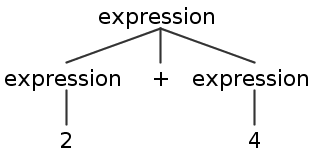
\includegraphics[scale=0.4]{pics/antlr4_parse_tree_visitAdditionVisitNumberBeispiel.png}
\caption{Syntaxbaum für beispielhaften arithmetischen Ausdruck}
\end{figure}
\pagebreak
Zunächst wird die visitAddition-Methode aufgerufen, da der Operator der expression das ''+'' Zeichen ist. Die visitChildren-Methode gibt nun die Zeichenkette
\begin{lstlisting} [frame=single]
ldc 2
ldc 4
\end{lstlisting}
zurück, da die untergeordneten Expressions nur Zahlen enthalten. Dem fügt die visitAddition-Methode wiederrum den Befehl
\begin{lstlisting} [frame=single]
iadd
\end{lstlisting}
hinzu, um die Addition durchzuführen.
\linebreak

In der JavaVM werden diese Instruktionen wie folgt verarbeitet:
Im Initialzustand ist der Stack leer.

\begin{figure}[h!]
\centering

\includegraphics[scale=0.2]{pics/stack_visual.png}
\caption{Zustand des Kellerspeicher der JavaVM}
\end{figure}

Der Befehl \textit{ldc 2} legt den Wert \textit{2} auf den Stack.

\begin{figure}[h!]
\centering

\includegraphics[scale=0.2]{pics/stack_visual(1).png}
\caption{Zustand des Kellerspeicher der JavaVM}
\end{figure}

Der Befehl \textit{ldc 4} legt den Wert \textit{4} auf den Stack.

\begin{figure}[h!]
\centering

\includegraphics[scale=0.2]{pics/stack_visual(2).png}
\caption{Zustand des Kellerspeicher der JavaVM}
\end{figure}

Der Befehl \textit{iadd} nimmt zwei Werte vom Stack und legt das Ergebnis der Addition dieser Werte wieder auf den Stack

\begin{figure}[h!]
\centering

\includegraphics[scale=0.2]{pics/stack_visual(3).png}
\caption{Zustand des Kellerspeicher der JavaVM}
\label{fig:method}
\end{figure}



\pagebreak

\subsection{Ausweiten der simplen Grammatik}
Nachdem die Sprache grundlegende Funktionalität erhielt, versuchten wir die weiteren Bestandteile, die durch die Anforderungen festgelegt wurden, zu implementieren. 


\subsubsection{Ergebnisausgabe}
Ein Programm ohne Ausgabe ergibt keinen Sinn, da nie das berechnete Ergebnis betrachtet werden kann. Eine Ausgabefunktion zu implementieren stellte sich nicht als all zu großes Problem heraus, da Jasmin die Fähigkeit besitzt Objekte und Methoden in der Java Library zu nutzen. Wir implementierten dies Ausgabefunktion wie folgt:

\scriptsize \begin{lstlisting}[frame=single]
/**@brief
 * vearbeitet den Aufruf der println-Funktion
 */
public String visitPrintln(PrintlnContext ctx) {
	return  ";calling println\n" + 
		//legt ein System.out Objekt auf den Stack
		"getstatic java/lang/System/out Ljava/io/PrintStream;\n" + 	
		//Argument der print-Funktion
		visit(ctx.argument) + 						
		//ruft die Methode println des System.out-Objekts auf
		"invokevirtual java/io/PrintStream/println(I)V\n\n"; 				
}
\end{lstlisting}

\normalsize
Es wird zuerst ein System.out-Objekt auf den Stack gelegt, danach der auszugebende Wert. Schließlich folgt der Aufruf der Methode println(), die das Argument sowie das System.out-Objekt vom Stack wieder herunternimmt.


Der Aufruf in unserer Programmiersprache lautet: 
\begin{lstlisting}[frame=single]
println( argument );
\end{lstlisting}

\subsection{Implementierung von Variablen}
Eine Variable wird folgendermaßen deklariert:
\begin{lstlisting}[frame=single]
int NAME;
\end{lstlisting}
Wenn ein entsprechender Knoten im Syntaxbaum besucht wird, wird geprüft, ob bereits eine Variable mit dem selben Namen im aktuellen Gültigkeitsbereich existiert. Ist dies der Fall, wird eine Exception ausgelöst und der Kompiliervorgang mit einer entsprechenden Fehlermeldung beendet. Existiert der Name der Variablen im aktuellen Gültigkeitsbereich noch nicht wird ein neuer Eintrag in der Variablentabelle erstellt.

Um einer deklarierten Variable einen Wert zuzuweisen, wird folgende Syntax verwendet:
\begin{lstlisting}[frame=single]
NAME = EXPRESSION;
\end{lstlisting}
Dabei muss eine EXPRESSION zu einem Wert evaluierbar sein.
Wird ein Knoten mit einer Zuweisung besucht, erfolgt zuerst der Versuch den Namen der Variablen zu einem Index in der Variablentabelle aufzulösen. Gelingt dies nicht, bedeutet das, dass die Variable nicht deklariert wurde. Es wird eine enstprechende Exception ausgelöst. Kann der Name der Variablen zu einem Index aufgelöst werden, wird der Wert der Variable mit 
\begin{lstlisting}[frame=single]
istore [index]
\end{lstlisting}
vom Stack genommen und in der Jasmin-Variablentabelle gespeichert.

Wird auf eine Variable lesend zugegriffen, d.h. sie kommt im rechten Teil einer Zuweisung vor, so muss auch wieder der Name zu einem Index aufgelöst werden. Hierzu wird intern die gleiche Methode verwendet. Nach erfolgreichem Ermitteln des Index kann der Wert der Variable mit dem Befehl 
\begin{lstlisting}[frame=single]
iload [index]
\end{lstlisting}
wieder auf den Stack gelegt und somit verwendet werden.

\subsection{Implementierung von Funktionen}
Vor dem eigentlichen Aufruf des Visitors, wird der gesamte Baum auf Funktionsdeklarationen untersucht. Dies sorgt dafür, dass Funktionen an beliebigen Stellen im Quellcode definiert werden können und keine Vorwärtsdeklarationen notwendig sind. Die gefundenen Funktionen werden in einer Liste gespeichert.

%Funktionen werden mit folgender Syntax deklariert:
% ToDo: Bitte einfügen; 
%	siehe Kapitel Verwendung

Wird ein Knoten mit einer Funktionsdeklaration besucht wird zunächst in dieser Liste überprüft, ob eine Funktion mit der gleichen Signatur bereits existiert. Ist dies der Fall, wird eine Exception ausgelöst und der Kompiliervorgang abgebrochen. Andernfalls wird ein neuer Eintrag mit dem Namen und der Signatur der Funktion in die Funktionsliste eingefügt.
Die Signatur besteht dabei aus dem Namen und den übergebenen Parametern. Beispielsweise dürfen sowohl die Funktion
\begin{lstlisting}[frame=single]
int doSomething();
\end{lstlisting}
als auch die Funktionen
\begin{lstlisting}[frame=single]
int doSomething(int paramA);
int doSomething(int paramA, int paramB);
\end{lstlisting}
in der gleichen Quelldatei vorkommen, da sie sich in den Übergabeparametern unterscheiden.

Beim Aufruf von Funktionen wird ebenfalls geprüft, ob eine Funktion mit der gegebenen Signatur existiert. Existiert die Funktion nicht, wird eine Exception ausgelöst, andernfalls der Funktionsaufruf wie folgt verarbeitet. 
In einem String wird die Anweisungen für den Aufruf für Jasmin zusammengesetzt, wobei zunächst gegebenenfalls Variablen für die Übergabeparameter angelegt werden. 
Anschließend wird der Aufruf in Jasmin-Syntax generiert.

\begin{lstlisting}[frame=single]
invokestatic [objektname]/[funktionsname]([parameter])[rückgabetyp]
\end{lstlisting}
Der Objektname ist nur intern, also für die JVM relevant, da diese der Java-Philosophie entsprechend stark objektorientiert ausgerichtet ist. Es muss also nur darauf geachtet werden, dass der Objektname gleich dem der Jasmin-Main-Funktion ist.
Die Parameterliste besteht aus je einem ''I'' (für Integer) pro übergebenem Parameter.
Der Rückgabetyp wird wiederrum durch ein ''I'' für den Datentyp Integer angegeben. Da der einzige unterstützte Datentyp unserer Sprache ''int'' ist, ist der Rückgabetyp hardcodiert und damit für jede Funktion gleich.

Desweiteren wird bei einem Funktionsaufruf die aktuelle Variablentabelle kopiert und eine neue Variablentabelle für die Funktion angelegt. Dies ermöglicht verschiedene Gültigkeitsbereiche (engl. scopes). 
Beim Verlassen der Funktion wird die vorherige Variablentabelle wieder hergestellt.

\subsection{Implementierung von Konstanten}
Konstanten sind intern als Erweiterung von Variablen anzusehen. 
Zusätzlich zu Variablen werden bei Konstanten folgende Schritte ausgeführt:
Wird eine Konstante deklariert, wird deren hasBeenAssigned-Flag auf false gesetzt.
Bei der Wertzuweisung zu der Konstanten wird geprüft, welchen Wert dieses Flag besitzt. Ist der Wert false, wird eine normale Zuweisung durchgeführt und der Wert des Flags auf true gesetzt. Ist der Wert true, wurde der Konstanten bereits eine Wert zugewiesen, weshalb eine weitere Zuweisung nicht erfolgen darf. Es wird eine Exception ausgelöst und der Kompiliervorgang mit einer entsprechenden Fehlermeldung abgebrochen.

\subsection{Implementierung von Bedingten Verzweigungen}
Verzweigungen sind in drei Teile untergliedert:
\begin{itemize}
	\item conditionInstructions
	\item onTrueInstructions
	\item onFalseInstructions	
\end{itemize}

Die conditionInstructions enthalten die Auswertung eines mathematischen Ausdrucks, dessen Ergebnis einen Wahrheitswert repräsentiert. Der Wert 0 repräsentiert \textit{false}, alle anderen Werte werden als \textit{true} interpretiert.
 
Wird die Bedingung zu true evaluiert, werden die onTrueInstructions ausgeführt, die onFalseInstructions werden übersprungen. Andernfalls, werden die onTrueInstructions übersprungen und die onFalseInstructions ausgeführt.
Um die entsprechenden Instruktionen zu überspringen, werden Labels benötigt, die einen Sprung zu einer definierten Stelle im Proramm ermöglichen. Damit die Labels für jede Verzweigung eindeutig sind, wird gezählt, wie oft Verzweigungen vorkommen und die Labels entsprechend benannt.

\subsection{Implementierung einer Schleife}
Eine Schleife wird intern  in
\begin{itemize}
\item Bedingung
\item Befehle, die bei einer wahren Bedingung ausgeführt werden
\end{itemize}

Der folgende Pseudocode ist ähnlich zu entsprechenden Jasmin-Anweisungen :
\\
\begin{algorithm}[H]
	conditionLabel \\
	conditionInstructions \\
		\If{conditionInstructions == true}
		{ 
			Sprung zu onTrueLabel
		}
		\If{conditionInstruction == false}
		{
			Sprung zu endOfWhileLabel
		}
	[onTrueLabel] \\
	onTrueInstructions \\
	Sprung zu conditionLabel \\	
	endOfWhileLabel
\end{algorithm}
\(\)\\
Die Labels werden benötigt, damit in der Schleife an die entsprechende Stelle gesprungen werden kann. Damit intern die Labels zur richtigen Schleife zugeordnet werden können, wird mitgezählt, wie oft Schleifen im Programm verwendet werden.

\subsection{Dokumentation}
Zur effizienten Erstellung der Dokumentation wurde \LaTeX \(\) in Verbindung mit TexMaker verwendet. Dazu wurden die einzelnen Hauptüberschriften in eigene Dateien ausgelagert und in der Hauptdatei inkludiert. Dies hat eine erhöhte Übersichtlichkeit zur Folge.
Um die Dokumentation versioniert zu speichern, wurde diese im verwendeten Git-Repository hochgeladen. Damit keine unnötigen Entwicklungs- bzw. Zwischenschrittdateien von \LaTeX \(\) in das verwendete Git-Repository übernommen werden, wurde ein Alias erstellt, der ebendiese Dateien beim Alias-Aufruf automatisiert entfernt. Dieser Alias sieht wie folgt aus:

\begin{lstlisting}[frame=single]
rmtex_dev()
{
	echo "Removing .aux"
	rm *.aux &> /dev/null
	echo "Removing .toc"
	rm *.toc &> /dev/null
	echo "Removing .synctex.gz"
	rm *.synctex.gz &> /dev/null
	echo "Removing .log"
	em *.log &> /dev/null
	echo "Removing .out"
	rm *.out &> /dev/null
}
\end{lstlisting}
\pagebreak
% !TEX root = Main.tex

\section{Aufgetretene Probleme und deren Lösung}

\subsection{Probleme im Projekt und Team}
Neben den bereits in anderen Kapiteln genannten Problemen mit Werkzeugen wie \textit{Eclipse}, bestand auch eine große Barriere im Team in der Zeiteinteilung. So ergaben sich zum Beispiel unterschiedliche Arbeitszeiten und Zeitspannen, in denen am Projekt gearbeitet werden konnte, was Absprachen und Besprechungen in die Länge zieht und nach unserer Erfahrung sehr mühsam macht.

\subsection{Operatorenpriorität bei arithmetischen Ausdrücken}
vgl. Kapitel oben

\subsection{Variablen}
Ein wichtiger Bestandteil jeder Programmiersprache ist die Möglichkeit Variablen zu nutzen. Damit eine Variable im späteren Programmverlauf genutzt werden kann, muss sie zunächst deklariert werden. In unserer Sprache erfolgt dies durch die Angabe [Datentyp] [Name];. Beispielsweise legt der Aufruf

\begin{lstlisting}[frame=single]
int x;
\end{lstlisting}

eine Integer-Variable mit dem Namen x an.

Als nächstes sollte eine Wertzuweisung erfolgen:
\begin{lstlisting}[frame=single]
x = 42;
\end{lstlisting}

Nachdem diese obligatorischen Schritte vollzogen wurde, kann der Wert der Variable beliebig oft ausgelesen oder verändert werden.

Damit diese Features in die Zielsprache zu übertragen werden, nutzt unser Compiler eine Variablentabelle. Jasmin besitzt die Möglichkeit den Wert der oben auf dem Stack liegt zwischenzuspeichern. Der Befehl
\begin{lstlisting}[frame=single]
astore <var-num>
\end{lstlisting}
nimmt den Wert vom Stack und speichert in am Index <var-num> in der Variablentabelle.

Mit dem Befehl
\begin{lstlisting}[frame=single]
aload <var-num>
\end{lstlisting}
wird die Variable an der Position <var-num> wieder auf den Stack gelegt. 
Jasmin akzeptiert nur ganze Zahlen > 0, jedoch keine Zeichenketten, für <var-num>
Deshalb muss unser Compiler den Variablenname, den der Nutzer der Sprache wählt, zu einem Index auflösen.

\subsubsection{Redefinition von bereits definierte Variable}
Wenn im Syntaxbaum eine Variablendeklaration gefunden wird, wird zunächst überprüft, ob eine Variable mit diesem Namen bereits vorhanden ist. Für diesen Abgleich wird intern eine HashMap verwendet. Ist der Name noch nicht vorhanden, wird er der HashMap hinzugefügt, wobei der Schlüssel der Name der Variable und der Wert die aktuelle Größe der Tabelle ist. Dies ist notwendig, um den Jasmin-Befehlen \textit{astore} und \textit{aload} einen Index  zu übergeben.

\subsubsection{Zugriff auf undefinierte Variable}
Ein möglicher Fehler seitens des Benutzer unserer Sprache ist, dass eine Variable aufgerufen wird, obwohl diese zuvor nicht definiert wurde. Beim Aufruf einer Variablen wird deshalb zunächst überprüft, ob diese in der Variablen-Map vorhanden ist. Falls nicht wird eine entsprechende Exception ausgelöst.


\subsection{Funktionen}
\subsubsection{Zugriff auf undefinierte Funktion}
\subsection{Redefinition von bereits definierten Funktion}
\subsubsection{Gültigkeitsbereiche}
\subsubsection{Funktionen mit gleichem Namen und unterschiedlichen Signaturen}
\subsection{Vorwärtsdeklarationen}

\subsection{Bedingte Verzweigungen}
\subsubsection{Umsetzung in Jasmin mit Hilfe von Labels und Sprungbefehlen}



\pagebreak
% !TEX root = Main.tex

\section{Verwendung der UnsereCompilerbauSprache}
Ein gültiges Programm in der UnsereCompilerbauSprache besteht aus beliebig vielen Statements und Funktionsdefinitionen. 

\subsection{Datentypen}
Der einzige Datentyp der Sprache ist 'int'. Ein 'int' repräsentiert eine ganze Zahl mit einer Größe von 32 bit. Mögliche Werte liegen zwischen -2147483648 und 2147483647 ($-2^{31}$ bis $2^{31} - 1$). %das hat doch nix mit zuweisung zu tun?! der wertebereich ändert sich ja nicht dadurch dass es eine bzw. keine zuweisung ist 

\subsection{Bezeichner}
Bezeichner werden genutzt, um Variablen, Konstanten sowie Funktionen zu benennen.
Bezeichner müssen eindeutig sein, d.h. ein Bezeichner darf im entsprechenden Gültigkeitsbereich in nur einer Deklaration des gleichen Typ vorkommen. Gültige Bezeichner beginnen mit einem Klein- oder Großbuchstaben und dürfen von beliebig vielen weiteren Klein- bzw. Großbuchstaben sowie den Ziffern von 0 bis 9 gefolgt werden. Ein Bezeichner darf kein reserviertes Schlüsselwort sein (vgl. Liste der reservierten Schlüsselwörter).

\subsection{Numerische Werte}
Numerische Werte bestehen aus einer beliebig langen Folge der Ziffern von 0 bis 9. Ein numerischer Wert muss aus mindestens einer Ziffer bestehen.

\subsection{Besondere Formatierungszeichen} 
Leerzeichen, Tabulatoren sowie Zeilenumbrüche dürfen in einer Quelltext-Datei vorkommen, werden jedoch vom Compiler ignoriert.

\subsection{Statements}
Alle Statements außer if-else-Anweisungen und Schleifen werden mit einem Semikolon '';'' beendet.
%eine halbe seite weiter oben steht, dass eine funktionsdeklaration KEIN statement ist...

\subsection{Variablen}
\subsubsection{Deklaration}
Variablen werden mit dem Schlüsselwort \textit{int} sowie dem gewünschten Namen nach einem Leerzeichen deklariert.
Der Name wird durch einen Bezeichner angegeben.

Beispiel:
\begin{lstlisting} [frame=single] 
int beispiel;
\end{lstlisting}

\subsubsection{Definition}
Nach dem eine Variable deklariert wurde, kann ihr ein Wert zugewiesen werden. Eine Zuweisung erfolgt durch das Gleichheitszeichen ''=''. Die linke Seite der Zuwesiung ist dabei der Name der Variable, die rechte Seite  kann ein arithmetischer Ausdruck, der Aufruf einer Funktion, eine Variable oder eine Konstante sein.
Wertzuweisungen von Variablen dürfen beliebig oft erfolgen.
Die Zuweisung muss getrennt von der Deklaration erfolgen.

Beispiel:
\begin{lstlisting} [frame=single] 
beispiel = 42;
beispiel = eineFunktion();
beispiel = 1 + 2 + 3;
beispiel = eineAndereVariable;
beispiel = EINEKONSTANTE;
\end{lstlisting}
%identifier können keine underscores enhalten


\subsubsection{Aufruf}
Variablen dürfen auch in der rechten Seite einer Zuweisung vorkommen.
Beispiel:
\begin{lstlisting} [frame=single] 
int beispiel1;
int beispiel2;

beispiel1 = 42;
beispiel2 = beispiel1 - 1;
\end{lstlisting}


\subsection{Konstanten}
Konstanten werden ähnlich wie Variablen verwendet.

\subsubsection{Deklaration}
Im Gegensatz zu einer Variablen wird dem Namen das Schlüsselwort \textit{const int} anstatt nur \textit{int} vorgestellt.

Beispiel:
\begin{lstlisting} [frame=single] 
const int BEISPIEL;
\end{lstlisting}

\subsubsection{Definition}
Die Wertzuweisung erfolgt wie bei einer Variable, darf jedoch nur ein mal pro Konstante erfolgen.
 

\subsection{Ergebnisausgabe}
Mit Hilfe der Funktion \textit{println([argument])} können numerische Werte, arithmetische Ausdrücke, logische Ausdrücke, Vergleiche, Rückgabewerte von Funktionen, Variablen und Konstanten auf die Konsole ausgegeben werden.

Beispiele:
\begin{lstlisting} [frame=single] 
int beispiel;
const int BEISPIEL;

beispiel = 42;
BEISPIEL = 123;

println(42);
println(42*5);
println(42<5);
println(42<5 && beispiel==BEISPIEL);
println(testFunktion(42));
println(beispiel);
println(BEISPIEL);
\end{lstlisting}


\subsection{Funktionen}

\subsubsection{Deklaration}
Funktionen könnnen an einer beliebigen Stelle im Quellcode deklariert werden. Ein Aufruf ist auch vor der Deklaration möglich.

Eine Funktionsdeklaration setzt sich folgendermaßen zusammen:
Schlüsselwort ''int'' für den Typ des Rückgabewerts, Bezeichner als Name der Funktion, öffnende runde Klammer, beliebig viele Variablendeklarationen (keine Übergabeparameter sind auch möglich), schließende runde Klammer und schließlich ein Funktionsrumpf.
Der Funktionsrump beginnt mit einer öffnenden geschweiften Klammer gefolgt von beliebig vielen Statements. 
Ein besonderes Statement ist die Rückgabe. Beim Auruf von \textit{return} wird die Funktion verlassen. Wenn hinter \textit{return} ein numerischer Wert, eine Variable, eine Konstante, ein arithmetischer Ausdruck, ein logischer Ausdruck oder der Aufruf einer weiteren Funktion folgt, so stellt dies den Rückgabewert der Funktion dar.
Der Funktionsrumpf wird mit einer schließenden geschweiften Klammer abgschlossen.

Beispiel:
\begin{lstlisting} [frame=single] 
int add(int a, int b) {
	println(a);
	println(b);
	return a + b;
}
\end{lstlisting}

\subsubsection{Aufruf}
Funktionsaufrufe dürfen in der rechten Seite von Zuweisungen, als Argument für die println-Funktion und als Teil von logischen sowie arithmetischen Ausdrücken vorkommen. Funktionsaufrufe dürfen auch eigenständige Statements sein.

Ein Funktionsaufruf setzt sich wie folgt zusammen:
[nameDerFunktion]([Parameterliste])

Die Funktion wird beim Verlassen mit dem zuvor definierten Rückgabewert substituiert.

Beispiel;
\begin{lstlisting} [frame=single] 
int x;
int y;
int z;

x = 40;
y = 2;
z = add(x, y);
\end{lstlisting}

\subsection{Arithmetik}
Arithmetische Ausdrücke dürfen folgende Komponenten besitzen:

\subsubsection{Operationen}
Jede Operation setzt sich aus einem linken Operanden, einem Operator sowie einem rechten Operanden zusammen.

Zulässige Operationen sind:
\begin{center}
  \begin{tabular}{ | c | c | }
    \hline
    Operator & Operation\\ \hline \hline
    + & Additionen\\ \hline
    - & Subtraktionen\\ \hline
    * & Multiplikationen\\ \hline
    / & Divisionen\\ \hline
  \end{tabular}
\end{center}
Die Operationen sind hier in aufsteigender Bindung aufgelistet, d.h., dass beispielsweise eine Division eine höhere Bindung als eine Addition besitzt. (Umgangssprachlich ''Punkt vor Strich'')

\paragraph{Operanden}
Zulässige Operanden für aritmetische Operationen sind:

\begin{list}{•}
\item numerische Werte \item
\item Variablen
\item Konstanten
\item Funktionen (bzw. deren Rückgabewerte)
\item weitere Operationen
\end{list}

Aus dem letzten Eintrag dieser Liste ergibt sich eine Rekursion, die eine beliebige Länge von arithmetischen Ausdrücken ermöglicht.

\paragraph{Klammerung}
Operationen dürfen Klammern mit beliebiger Verschachtelungstiefe enthalten.
Geklammerte Terme besitzen die höchst mögliche Bindung, d.h. höher als eine Division.

\subsection{Aussagenlogik}
Logische Ausdrücke werden wie in C intern als ''integer'' gespeichert und besitzen keinen eigenen Datentyp. Dabei repräsentiert der Wert 0 den Wahrheitswert \textit{false}, alle anderen Werte gelten als \textit{true}. Wie auch arithmetische Ausdrücke, dürfen logische Ausdrücke eine beliebige Länge besitzen und eine beliebig tiefe Klammerschachtelung besitzen.

Logische Ausdrücke werden verwendet, um Bedingungen auszudrücken, also in if-else-statements sowie in Schleifen.

Folgende Operationen stehen dafür in dieser Priorität zur Verfügung:
\begin{center}
  \begin{tabular}{ | c | c | c | }
    \hline
    Operation & Operator & Ergebnis\\ \hline \hline
    Konjunktion & \& \& & Wahr, wenn beide Operanden wahr sind. Sonst false.\\ \hline
    Disjunktion & || & Wahr, wenn ein oder beide Operanden wahr sind. \\ 
	& & Sonst false.\\ \hline
    Negation & ! & Das Gegenteil das negierten Term.\\ \hline   
  \end{tabular}
\end{center}

Desweiteren stehen folgende Vergleichsoperationen zur Verfügung:
\begin{center}
  \begin{tabular}{ | c | c | }
    \hline
    Operator & Vergleich\\ \hline \hline
    < & kleiner als\\ \hline
    <= & kleiner als oder gleich\\ \hline
    > & größer als\\ \hline
    >= & größer als oder gleich\\ \hline    
    == & gleich\\ \hline    
  \end{tabular}
\end{center}
Wenn ein Vergleich eine wahre Aussage ist, ist das Ergebnis des Vergleich \textit{true}.
Wenn ein Vergleich eine falsche Aussage ist, ist das Ergebnis \textit{false}.

\subsection{Bedingte Verzweigungen}
Eine bedingte Verzweigung ist ein Programmabschnitt der abhängig von einer Bedingung ausgeführt oder ignoriert wird. Es ist ebenfalls möglich eine Alternative anzugeben, die nur ausgeführt wird, falls die Bedingung nicht erfüllt wird.

Eine bedingte Verzweigung beginnt mit dem Schlüsselwort \textit{if} gefolgt von einer Bedingung umschlossen von runden Klammern. Dabei muss die Bedingung ein logischer Ausdruck sein. Wenn die Bedingung zu \textit{true} evaluiert wird, werden die Statements, die umgeben von geschweiften Klammern auf die Bedingung folgen, ausgeführt. 
Optional dürfen anschlißend das Schlüsselwort \textit{else} sowie weitere Statements umschlossen von geschweiften Klammern folgen. Diese Anweisungen werden ausgeführt falls die Bedingung zu \textit{false} evaluiert wird. Der else-Teil darf auch ausgelassen werden.

Beispiel (nur if-Teil):
\begin{lstlisting} [frame=single] 
int x;
int y;

x = 42;
y = 3;

if(x > y) {
	println(x);
} 
\end{lstlisting}

Beispiel (vollständiges if-else-statement):
\begin{lstlisting} [frame=single] 
int x;
int y;

x = 42;
y = 3;

if(x > y) {
	println(x);
} else {
	println(y);
}
\end{lstlisting}

\subsection{Schleifen}
Eine Schleife beginnt mit dem Schlüsselwort \textit{while}, wird von einer Bedingung in runden Klammern gefolgt und schließt mit einem Schleifenrumpf ab. Der Schleifenrumpf wiederrum wird mit geschweiften Klammern geöffnet und abgeschlossen.

Sowohl beim ersten Aufruf der Schleife als nach jedem Schleifendurchlauf wird überprüft, ob die gegebenene Bedingung wahr oder falsch ist. Ist die Bedingung wahr, werden die Anweisungen im Schleifenrumpf ausgeführt. Falls die Bedingung falsch ist, werden die Anweisungen nicht ausgeührt.



Beispiel (gibt die Summer der Zahlen von 1 bis 10 aus):
\begin{lstlisting} [frame=single] 
int i;
int x;

i = 0;
x = 0;

while(i <= 10) {
	i = i + 1;
	x = x + i;
}
println(x);
\end{lstlisting}
	
\subsection{Reservierte Schlüsselwörter und Symbole}	

\begin{center}
  \begin{tabular}{ | c | c | }
    \hline
    Schlüsselwort & Bedeutung\\ \hline \hline
    int & Deklariert eine Variable\\ \hline
    const int & Deklariert eine Konstante\\ \hline
    println & Aufruf der Ausgabefunktion\\ \hline
    return & Hinter ''return'' folgt der Rückgabewert einer Funktion\\ \hline
    if & Beginn eines if(-else)-Statements\\ \hline
    else & Beginn des else-Teil eines if-else-Statements\\ \hline
    while & Beginn einer while-Schleife\\ \hline
    
  \end{tabular}
\end{center}


\begin{center}
  \begin{tabular}{ | c | c | }
    \hline
    Symbol & Bedeutung\\ \hline \hline
    = & Zuweisungsoperator\\ \hline
    + & Operator für Additionen\\ \hline
    - & Operator für Subtraktionen\\ \hline
    * & Operator für Multiplikationen\\ \hline
    / & Operator für Divisionen\\ \hline
    
    < & Vergleichsoperator für kleiner als\\ \hline
    <= & Vergleichsoperator für kleiner gleich\\ \hline
    > & Vergleichsoperator für größer als\\ \hline
    >= & Vergleichsoperator für größer gleich\\ \hline    
    == & Operator um zwei Werte auf Gleichheit zu überprüfen\\ \hline    
    
    \& \&  & logisches Und \\ \hline    
    || & logisches Oder (inklusiv) \\ \hline    
    ! & logisches Nicht \\ \hline    
    
  \end{tabular}
\end{center}

\subsection{Beispielprogramm}

\begin{lstlisting} [frame=single]
int zahl1;
zahl1 = -4;

int zahl2;
zahl2 = 9;

int enumerator;
enumerator = 0;

const int zahl3;
zahl3 = 9;

if(zahl1 > zahl3)
{
	println(zahl1);
}
else
{
	println(zahl3);
}

while(enumerator < zahl2)
{
	println(enumerator);
	enumerator = enumerator + 1;
}

println(funktion(zahl3));
println(zahl3);

int funktion(int x)
{
	x = x+1;
	return x;
}
\end{lstlisting}

Dieses Programm kann mit dem im Projekt entwickelten Compiler übersetzt werden. Beim Betrachten diese Quellcodes werden einige Besonderheiten verdeutlicht.
\\
Zunächst ist zu beachten, dass Variablen nicht in einer Anweisung deklariert und initialisiert werden können. Folgende Schreibweise ist also ungültig: 
\begin{lstlisting} [frame=single]
int x = 4;
\end{lstlisting}
Stattdessen müssen die Initialisierung und Deklaration von Variablen in zwei Schritten durchgeführt werden:
\begin{lstlisting} [frame=single]
int x;
x = 4;
\end{lstlisting}

Bei der Verwendung von println muss auf den Funktionsnamen sofort die geklammerte Parameterliste folgen. Leerzeichen und sonstige andere Zeichen sind zwischen println und der geklammerten Parameterliste ungültig.
\\
Weiterhin fällt auf, dass Vorwärtsdeklarationen von Funktionen nicht notwendig sind.

\section{Aufruf des UnserCompilerbauCompilers}
Um eine Textdatei mit Anweisungen in der UCBS zu übersetzen, muss folgender Aufruf auf der Kommandozeilenebene erfolgen:
\begin{lstlisting} [frame=single]
java -jar UCC.jar sourceCode.txt 
\end{lstlisting}
Die Ausgabedatei tpblcOut.class kann nun mit Hilfe der JRE ausgeführt werden.
\begin{lstlisting} [frame=single]
java tpblcOut
\end{lstlisting}

\pagebreak
\section{Anhang}
Alle Dateien oder sonstige Dokumente, auf die sich in dieser Dokumentation bezogen wurden, sind in folgendem Git-Repository zu finden: \\
\href{https://github.com/nohoffmann/UnserCompilerbauCompiler}{https://github.com/nohoffmann/UnserCompilerbauCompiler}
\pagebreak
\end{document}
